\documentclass[tikz,border=10pt]{standalone}
\usepackage{amsmath}
\usetikzlibrary{arrows.meta, positioning, calc, decorations.pathreplacing}
\definecolor{c1}{HTML}{000000}
\definecolor{c2}{HTML}{233D4D}
\definecolor{c3}{HTML}{FE7F2D}
\definecolor{c4}{HTML}{EAECF0}
\definecolor{axiscolor}{HTML}{333333}
\definecolor{labelcolor}{HTML}{5F6B75}
\begin{document}
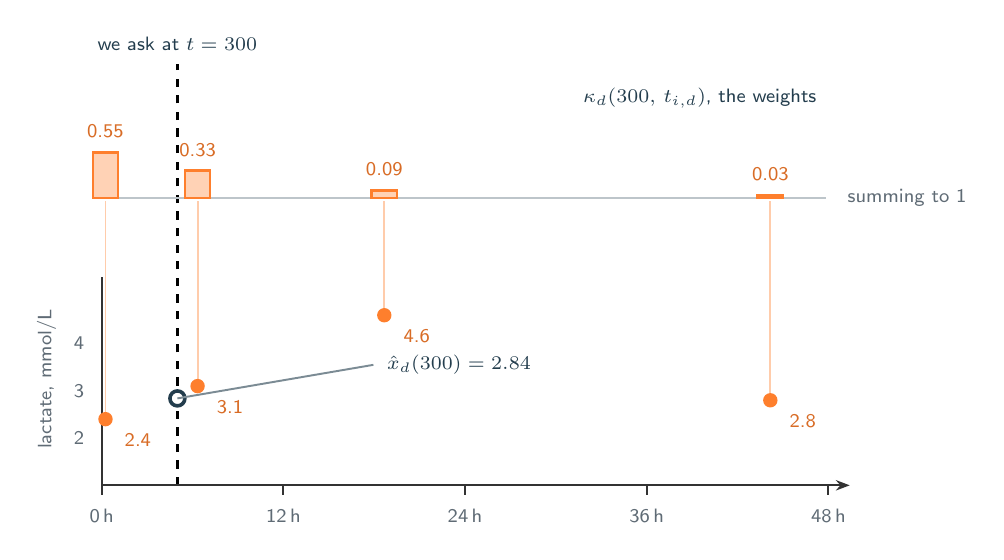
\begin{tikzpicture}[
    every node/.style={font=\sffamily},
    lab/.style={font=\sffamily\scriptsize, text=labelcolor},
    tag/.style={font=\sffamily\scriptsize, text=c2},
    hot/.style={font=\sffamily\scriptsize, text=c3!85!black},
]
\def\X#1{1.60 + #1*0.003200}
\def\Y#1{1.30 + (#1-2.0)*0.60}

% the query time, all the way up
\draw[c1, line width=0.9pt, dashed] ({\X{300}}, 0.70) -- ({\X{300}}, 6.05);
\node[tag, anchor=south] at ({\X{300}}, 6.10) {we ask at $t = 300$};

% ---------------- weights
\node[tag, anchor=east] at (10.80, 5.62) {$\kappa_d(300,\, t_{i,d})$, the weights};
\draw[c2!30, line width=0.6pt] (1.60, 4.35) -- (10.80, 4.35);
\foreach \m/\k/\txt in {15/0.55/{0.55}, 380/0.33/{0.33}, 1120/0.09/{0.09}, 2650/0.03/{0.03}}{
    \filldraw[draw=c3, fill=c3!35, line width=0.9pt]
        ({\X{\m}-0.16}, 4.35) rectangle ({\X{\m}+0.16}, {4.35 + \k*1.05});
    \node[hot, anchor=south] at ({\X{\m}}, {4.41 + \k*1.05}) {\txt};
}
\node[lab, anchor=west] at (10.95, 4.35) {summing to 1};

% ---------------- observations
\node[lab, rotate=90] at (0.90, 2.05) {lactate, mmol/L};
\draw[axiscolor, line width=0.7pt] (1.60, 0.70) -- (1.60, 3.35);
\foreach \v in {2, 3, 4}{ \node[lab, anchor=east] at (1.50, {\Y{\v}}) {\v}; }
\foreach \m/\v in {15/2.4, 380/3.1, 1120/4.6, 2650/2.8}{
    \draw[c3!40, line width=0.7pt] ({\X{\m}}, {\Y{\v}}) -- ({\X{\m}}, 4.31);
    \fill[c3] ({\X{\m}}, {\Y{\v}}) circle (2.6pt);
}
\node[hot, anchor=north west] at ({\X{15}+0.12}, {\Y{2.4}-0.06}) {2.4};
\node[hot, anchor=north west] at ({\X{380}+0.12}, {\Y{3.1}-0.06}) {3.1};
\node[hot, anchor=north west] at ({\X{1120}+0.12}, {\Y{4.6}-0.06}) {4.6};
\node[hot, anchor=north west] at ({\X{2650}+0.12}, {\Y{2.8}-0.06}) {2.8};

% the answer
\fill[white] ({\X{300}}, {\Y{2.84}}) circle (2.7pt);
\draw[c2, line width=1.3pt] ({\X{300}}, {\Y{2.84}}) circle (2.7pt);
\draw[c2!60, line width=0.7pt] ({\X{300}}, {\Y{2.84}}) -- (5.05, {\Y{3.55}});
\node[tag, anchor=west] at (5.10, {\Y{3.55}}) {$\hat{x}_d(300) = 2.84$};

\draw[axiscolor, line width=0.8pt, -{Stealth[length=5pt]}] (1.60, 0.70) -- (11.10, 0.70);
\foreach \h in {0, 12, 24, 36, 48}{
    \pgfmathsetmacro\m{\h*60}
    \draw[axiscolor, line width=0.7pt] ({\X{\m}}, 0.70) -- ({\X{\m}}, 0.58);
    \node[lab, anchor=north] at ({\X{\m}}, 0.52) {\h\,h};
}
\end{tikzpicture}
\end{document}
